\documentclass[a4paper,14pt]{extreport}
\usepackage[utf8]{inputenc} % Set Encoding
\usepackage[T1,T2A]{fontenc}
\usepackage{fontspec} % Using custom fonts (requires -xelatex flag)
\usepackage[russian,english,ukrainian]{babel} % Using languages
\usepackage{geometry} % Set margins
\usepackage[raggedright]{titlesec} % For section modification
\usepackage{indentfirst} % Inserts indents in paragraphs
\usepackage{minted} % For code listing
\usepackage{graphicx} % For image insertions
\usepackage{float} % For positioning
\usepackage[section]{placeins}
\usepackage{fancyhdr}
\usepackage{caption}
\usepackage{enumitem} % List indents
\usepackage{chngcntr}
\usepackage[english,russian,ukrainian]{babel}
\usepackage[nottoc]{tocbibind}
\usepackage{color}
\usepackage{xpatch}
\definecolor{spot}{rgb}{0,0,0}
\usepackage[colorlinks,allcolors=spot,bookmarksopen=true,pdfstartview=FitH]{hyperref}
\usepackage{amsmath}

\counterwithout{section}{chapter}

\pagestyle{fancy}

\fancyhf{}
\fancyhead[R]{\thepage}
\renewcommand{\headrulewidth}{0pt}
\fancyheadoffset{0mm}
\fancyfootoffset{0mm}
\renewcommand{\headrulewidth}{0pt}
\renewcommand{\footrulewidth}{0pt}
\setlength{\headheight}{17.0pt}

\fancypagestyle{plain}{
    \fancyhf{}
    \rhead{\thepage}}


\pagenumbering{gobble}

\usemintedstyle{bw}

\geometry{
  a4paper,
  left=30mm,
  right=20mm,
  top=20mm,
  bottom=20mm
}

\DeclareCaptionLabelFormat{gostfigure}{Рисунок #2}
\DeclareCaptionLabelFormat{gosttable}{Таблиця #2}
\DeclareCaptionLabelSeparator{gost}{~---~}
\captionsetup{labelsep=gost}
\captionsetup[figure]{labelformat=gostfigure, justification=centering,
labelsep=gost}
\captionsetup[table]{labelformat=gosttable, labelsep=gost}

\setlength\parindent{2.5em}
\renewcommand{\baselinestretch}{2.0}
\linespread{1.3} % Set default line spacing

\setmainfont{Liberation Serif} % Set default font on Linux

\titleformat{\section}
{\normalfont}{\thesection}{1em}{}

\titleformat{\subsection}
{\normalfont}{\thesubsection}{1em}{}

\titleformat{\subsubsection}
{\normalfont}{\thesubsubsection}{1em}{}

\titleformat{\chapter}[block]
    {\filcenter\bfseries}
    {\thechapter}
    {1em}
    {\MakeUppercase}{}

\renewcommand{\headrulewidth}{0pt}

\titlespacing{\chapter}{0pt}{-30pt}{2em}
\titlespacing\section{0cm}{2em}{1ex}
\titlespacing\subsection{0cm}{1ex}{1ex}

\newcommand\chap[1]{%
  \chapter*{#1}%
  \addcontentsline{toc}{chapter}{\uppercase{#1}}}

\graphicspath{{./pics}}

\setlist[enumerate]{leftmargin=4em}

\begin{document}
\begin{titlepage}
	\centering
    Міністерство освіти і науки України
    
    Харківський національний університет радіоелектроніки
    \vspace{1cm}

    Факультет комп'ютерних наук
    \vspace{1cm}

    Кафедра штучного інтелекту

    \vspace{2cm}
    \uppercase{Реферат}
    \vspace{1cm}

    на тему <<Бот Dvango>>
    \vspace{1cm}

    з дисципліни <<Системи інтелектуальної обробки природно-мовної інформації>>

    \begin{flushleft}
    \vspace{4cm}
    \begin{minipage}[t]{8cm}
        Виконали ст. гр. ІТШІ-18-1:

        Соколенко Дмитро Олександрович

        Апраксін Антон Романович
    \end{minipage}
    \hfill
    \begin{minipage}[t]{6cm}
        Прийняв:\\
        проф. каф. ШІ Рябова Н. В.\\
        з оцінкою ``\rule{2cm}{0.15mm}''\\
        ``\rule{0.7cm}{0.15mm}''\rule{2cm}{0.15mm}20\rule{0.7cm}{0.15mm}р
    \end{minipage}
    \end{flushleft}
	\vfill

	{Харків \the\year{}}
\end{titlepage}
\pagenumbering{arabic}
\setcounter{page}{3}

\chap{Реферат}

\chap{Скорочення}
ГНМ -- Глибокі нейронні мережі

РНМ -- Рекурентні нейронні мережі

\newpage
\tableofcontents
\newpage


\chap{Вступ}


\chap{Основна частина}
\section{Аналіз предметної галузі}
% https://papers.nips.cc/paper/2014/file/a14ac55a4f27472c5d894ec1c3c743d2-Paper.pdf
Глибокі нейронні мережі (ГНМ) -- надзвичайно потужні моделі машинного навчання,
які досягають чудової точності у таких складних задачах, як
розпізнавання мови та візуальне розпізнавання об’єктів.
ГНМ є потужними, оскільки вони можуть виконувати
довільні паралельні обчислення за невелику кількість кроків.
Отже, хоча нейронні мережі пов’язані
зі звичайними статистичними моделями, вони вивчають складні
обчислення. Більше того, великі ГНМ можна навчати зі
зворотним розповсюдженням, коли мічений навчальний набір має
достатньо інформації для визначення параметрів мережі. Таким
чином, якщо існує параметр великого ГНМ, який досягає хороших
результатів (наприклад, оскільки люди можуть вирішити завдання
дуже швидко), зворотне розповсюдження знайде ці
параметри і вирішить проблему.

\subsection{Штучні нейронні мережі}
Штучна нейронна мережа побудована навколо біологічної метафори.
Будова первинної зорової кори відносно добре відома,
і вчені виграли Нобелівську премію з фізіології за відкриття в
1962 р. організації нейронів у перших кортикальних
шарах \cite{cortex-stuff}. Таким чином, в надзвичайно
спрощеному вигляді
мозку нейрони організовані шарами, кожен нейрон отримує
інформацію з попереднього шару, виконує дуже просте
обчислення і передає свій результат нейронам наступного
шару. Однак слід пам’ятати, що це лише метафора та джерело
натхнення: біологічні мережі мають набагато складніші
зв’язки, а математичні рівняння, що керують ними, також
є більш складними \cite{cortex-equations}.

\subsubsection{Перцептрон}
Перцептрони -- винайдені Френком Розенблаттом у 1957 році
\cite{rozenblatt}, є найпростішою
нейронною мережею, яка складається з $n$ кількості входів, лише одного
нейрона та одного виходу, де $n$ - кількість рис нашого набору
даних. Процес вираховухання результату класифікації починається
з обчислення зваженої суми
по формулі \ref{eq:perceptron1}.

\begin{equation}
    z = \sum^n_{i=1} x_i w_i + b
    \label{eq:perceptron1}
\end{equation}

де $w$ -- вектор дійсних ваг, $b$ -- зміщення.
Коефіцієнт зміщення зміщує межу прийняття рішення
від початку координат і не залежить від будь-якого
вхідного значення.

Потім на зваженій сумі використовується функція активації.

\begin{equation}
    \phi(z) = \begin{cases}
        0 ,& z \le w_0 \\
        1 ,& z > w_0 \\
    \end{cases}
    \label{eq:perceptron2}
\end{equation}

\subsubsection{Багатошаровий персептрон}
Перші персептрони містили лише один шар. Такі одношарові
архітектури занадто прості, щоб вони могли виконувати складні задачі,
і завдяки додаванню декількох шарів ми можемо розрахувати більш складні
функції. Таким чином, глибокі нейронні мережі використовують дуже
велику кількість шарів. За останні роки ці архітектури дозволили
отримати дуже вражаючі результати для розпізнавання зображень та
відео, а також для автоматичного перекладу текстів.

Багатошаровий персептрон добавляє концепцію
``прихованого шару''. Тут нейрони розташовані у наборі шарів,
і кожен шар містить деяку кількість однакових нейронів.
Кожен нейрон в одному шарі з'єднаний з кожним нейроном в наступному шарі;
ми говоримо, що мережа тісно пов’язана. Перший рівень - це вхідний шар,
і його нейрони приймають значення вхідних рис. 
Останній рівень є вихідним шаром, і він має один нейрон для
кожного значення, яке виводить мережа (тобто один нейрон
в разі регресії або двійкової
класифікації, або $K$  у випадку класифікації з $K$ класами).
Усі шари між ними відомі як приховані шари, тому що ми не знаємо
заздалегідь, що ці одиниці повинні обчислювати, і це потрібно
виявити під час навчання \cite{nn:multilayer-perceptrons}.

Обчислення, які робить багатошарова мережа з двома
прихованими шарами можна
представити у векторизованій формі так \cite{nn:multilayer-perceptrons}:

\begin{gather}
\begin{aligned}
    h^{(1)} &= \phi^{(1)}(W^{(1)}x + b^{(1)}) \\
    h^{(2)} &= \phi^{(1)}(W^{(1)}h^{(1)} + b^{(2)}) \\
    y &= \phi^{(1)}(W^{(1)}h^{(2)} + b^{(3)}) 
\end{aligned}
\end{gather}

Векторизована форма зазвичай використовується так як підсумовування
та індекси можуть бути громіздкими. Оскільки кожен шар містить
багато нейронів, ми представляємо активації всіх його нейронів
за допомогою вектора активації $h^{(l)}$. Оскільки для кожної пари
нейронів у двох послідовних шарах існує вага, можна представити
ваги кожного шару за допомогою вагової матриці $W^{(l)}$. Кожен шар також має вектор зміщення $b^{(l)}$.

\subsubsection{Навчання мереж}
Навчання нейронної мережі полягає у виборі ``найкращих'' можливих
ваг набору нейронів, що складають мережу. Таким чином,
необхідно вибрати значення цих ваг, щоб найкраще вирішити
завдання, що вивчаються за набором навчальних даних.

Процедура навчання, таким чином, полягає у модифікації ваг $w$,
таких, що для кожного $x$, мережа $f_w$ передбачає якомога
точніше їх асоціювання, тобто в кінці тренування $y \approx f_w(x)$.
Простий вибір -- мінімізувати суму $E(w)$ квадратів
помилок, які математично записують як

\begin{equation}
    \min_w E(w) = \sum (f_w(x) - y)^2
\end{equation}

Це відповідає задачі оптимізації, оскільки необхідно знайти
набір параметрів, який оптимізує певну ціль.
Це складна проблема, оскільки параметрів дуже багато, і ці
параметри, особливо параметри прихованих шарів, мають складний
вплив на результат. На щастя, існують ефективні математичні та
алгоритмічні методи для ефективного вирішення цього типу задач
оптимізації. Вони ще не повністю зрозумілі на теоретичному
рівні, і це дуже активна область досліджень. Ці методи
оптимізації модифікують ваги мережі, щоб покращити її та
зменшити помилку навчання $E(w)$. Математичне
правило для прийняття рішення щодо стратегії оновлення
ваги називається зворотним розповсюдженням \cite{nn:backpropagation}.

У методі зворотного розповсюдження помилки
використовується правило складної похідної.
Часткові похідні функції помилки відносно різних ваг та зміщень
зворотньо поширюються через багатошаровий персептрон.
Цей акт диференціації дає нам градієнт, або ландшафт помилок,
який дозволяє приблизитися до мінімуму помилки. Це робиться
за допомогою алгоритмів оптимізації на основі градієнта, таких
як стохастичний градієнтний спуск, Adam, Monentum та інші
\cite{gradient-descend}.

% Всі інші моделі нейронних мереж будуються тих самих принципах,
% на яких працюють
% багатошарові перцептрони.

\subsection{Рекурентні нейронні мережі}
% Для того щоб 

На відміну від звичайних перцептронів, рекурентні нейронні
мережі (РНМ)
беруть на вхід не лише значення поточного вхідного вектору,
але й те, що вони сприйняли раніше в часі.

\begin{figure}[H]
    \centering
    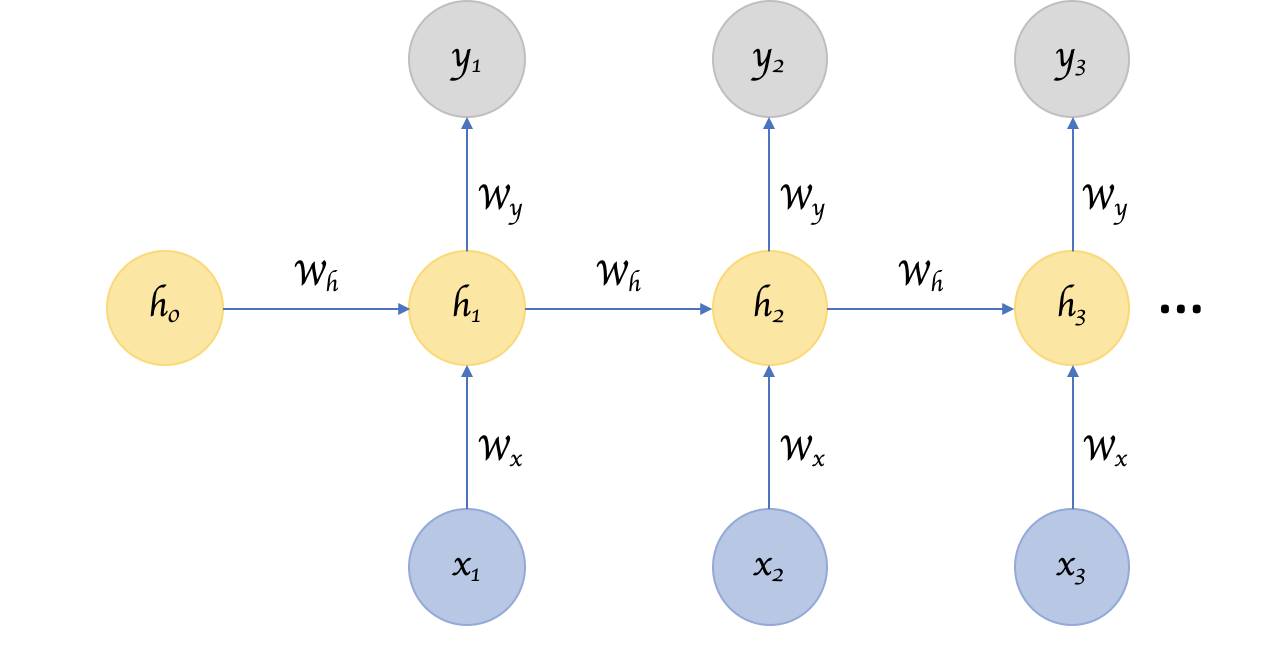
\includegraphics[width=0.75\textwidth]{recurrent-nn.png}
    \caption{Ілюстрація структури рекурентної нейронної мережі}
    \label{fig:rnn}
\end{figure}

Рішення рекурентної мережі, досягнуте на етапі часу $t-1$, впливає
на рішення, яке вона прийме через один шаг на етапі часу $t$.
Отже, рекурентні мережі мають два джерела вхідних даних -- поточні
та недавнє минуле, які разом визначають, як мережа
реагує на нові дані.

Можна сказати, що рекурентні зв'язки в нейронній мережі
дають можливість пам'ятати попередні рішення.
Додавання пам’яті до нейронних мереж має ціль: у самій послідовності
є інформація, і рекуррентні мережі використовують її для виконання
завдань, які мережі прямого зв'язку не можуть.
А саме, прихований стан дозволяє шукати
кореляційні залежності між подіями, розділеними багатьма моментами,
і ці кореляції називаються ``довгостроковими залежностями'',
оскільки подія за течією часу залежить і є функцією однієї
або кількох подій, що відбулися раніше.

Звичайна рекурентна одиниця описується формулами:

\begin{gather}
\begin{aligned}
    h_t &= \phi(W_h h_{t-1}+W_x x_t+b)\\
    y_t &= h_t
\end{aligned}
\end{gather}

Тут $x_t$ це вхід, $h_t$ -- рекурентна інформація, а $y_t$ -- 
результат на кроці $t$.

Однак рекурентні мережі, що складаються зі стандартних рекурентних
одиниць, не здатні обробляти довгострокові залежності: у міру
зростання розриву між відповідними входами важко
вивчити з'єднану інформацію. Основними причинами проблеми
довгострокових залежностей є те, що сигнали про помилки,
що надходять назад у часі, мають тенденцію або підірватися,
або зникнути \cite{nn:recurrent-hard}.

Для вирішення цієї проблеми було розроблено багато
методів, таких як LSTM \cite{nn:lstm}, GRU \cite{nn:gru}. Вони
гарно себе показали у задачах, які потребують захоплення
довгострокових залежностей. Такі задачі включають, але не обмежуються,
розпізнавання мови, машинний переклад.

Задачі, де завдання полягає у відображенні однієї послідовності в
іншу (машинний переклад, розпізнавання мови) становлять
виклик для рекурентних
нейронних мереж, оскільки вони вимагають, щоб розмірність
входів і виходів була відомою та фіксованою.
Для вирішення цієї проблеми була запропонована
модель ``seq2seq'' \cite{nn:seq2seq}. Загалом, вона спрямована
на перетворення вхідної послідовності (джерела) на нову (цільову),
і обидві послідовності можуть мати довільну довжину.
Приклади завдань трансформації включають машинний переклад
між кількома мовами як у тексті, так і в аудіо,
генерацію діалогу запитання-відповідь або навіть синтаксичний
розбір речень на дерева граматики.

Модель seq2seq зазвичай має архітектуру енкодер-декодер, що складається з:

\begin{enumerate}[label=--]
    \item Енкодер обробляє вхідну послідовність і стискає інформацію
    у контекстний вектор (також відомий як ембедінг речення
    або вектор ``думки'') фіксованої довжини. Очікується,
    що це відображення буде гарним підсумком значення
    цілої послідовності.
    \item Декодер ініціалізується контекстним вектором для
    виводу перетвореної послідовності. Ранні роботи
    використовували лише останній стан мережі
    енкодера як початковий стан декодера.
\end{enumerate}

І енкодер, і декодер є рекурентними нейронними мережами.

Критичним і очевидним недоліком цього дизайну контексту з
фіксованою довжиною є нездатність запам'ятовувати довгі речення.
Часто він забуває першу частину, як тільки завершує обробку всього
вводу. Для вирішення цієї проблеми народився
механізм уваги \cite{nn:attention}.

\subsection{Механізм уваги}
Увага до певної міри мотивована тим, як ми приділяємо зорову увагу
різним регіонам зображення або співвідносимо слова в одному реченні.

Зорова увага людини дозволяє зосередитись на певному регіоні з
``високою роздільною здатністю'', одночасно сприймаючи навколишнє
зображення в ``низькій роздільній здатності'', а потім відрегувати
фокусну точку або зробити відповідний висновок.
Враховуючи невеликий фрагмент зображення, пікселі в решті надають підказки, що
там відображається. Ми очікуємо побачити загострене вухо в жовтій коробці,
тому що ми бачили ніс собаки, ще одне загострене вухо праворуч і очі
Шіби (речі в червоних квадратах) (Рис. \ref{fig:shiba}). Однак
светр та ковдра внизу були
б не такими корисними, як ті собачі риси.

\begin{figure}[H]
    \centering
    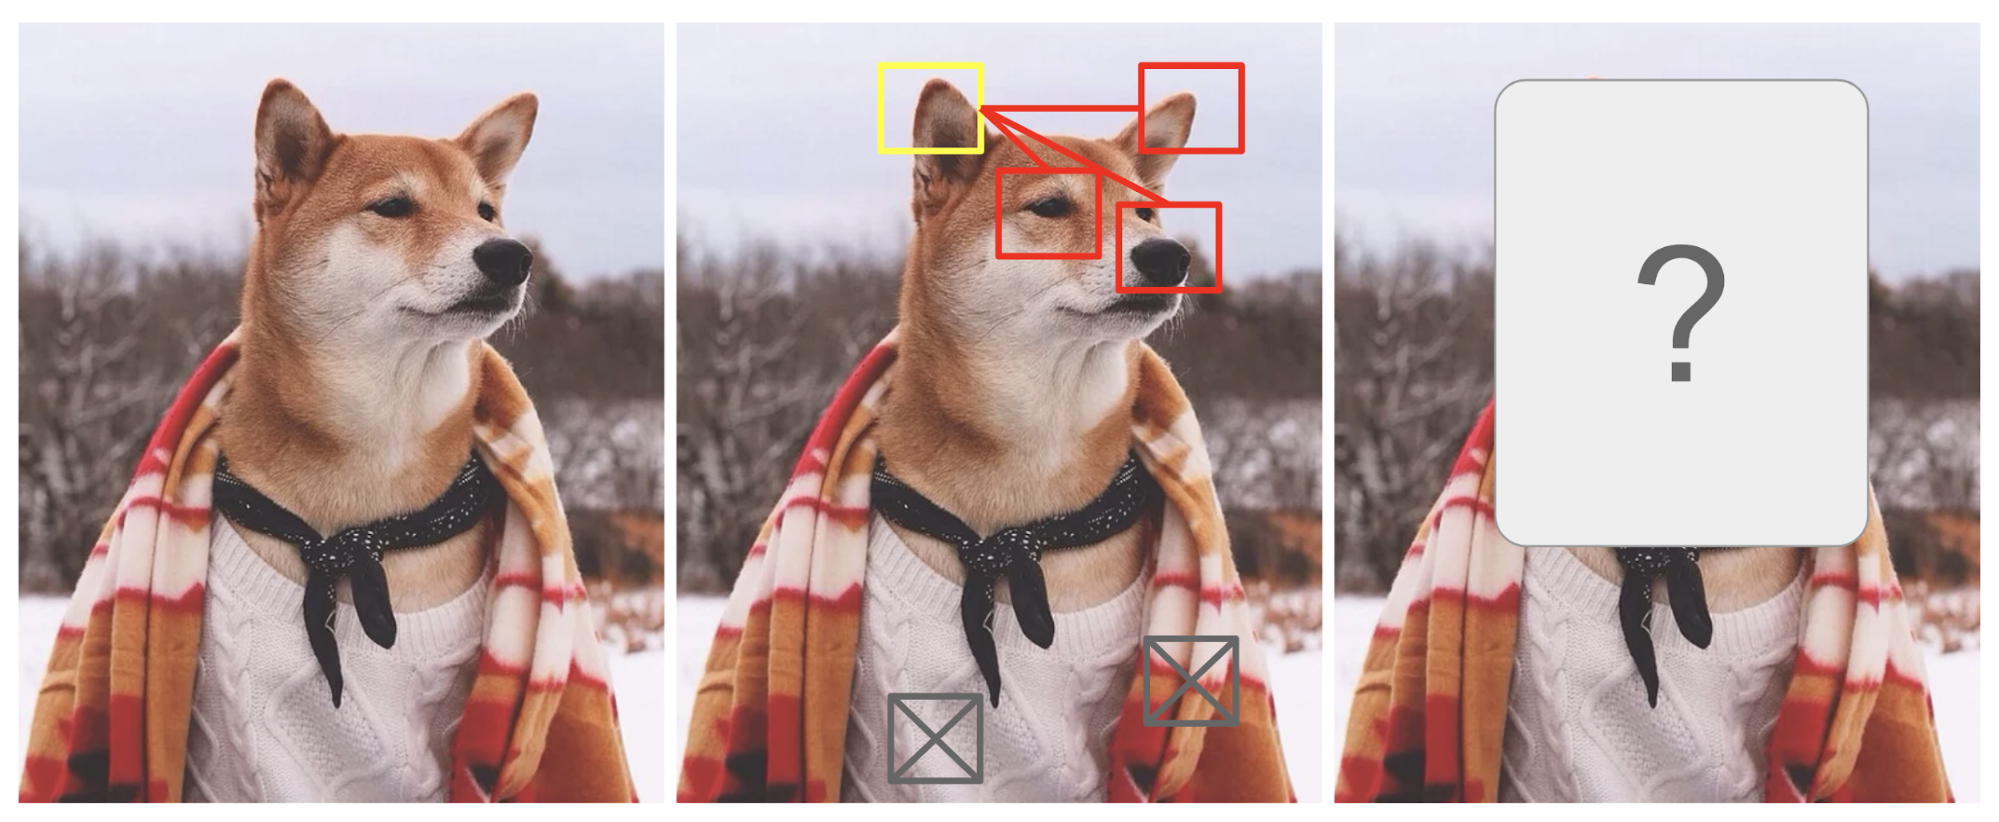
\includegraphics[width=0.75\textwidth]{shiba-example-attention.png}
    \caption{Шіба-іну в одязі}
    \label{fig:shiba}
\end{figure}

Подібним чином ми можемо пояснити зв'язок між словами в одному реченні
або близькому контексті. Коли ми бачимо ``їсти'', ми сподіваємось дуже
скоро зустріти слово, що означає вид їжи.

\begin{figure}[H]
    \centering
    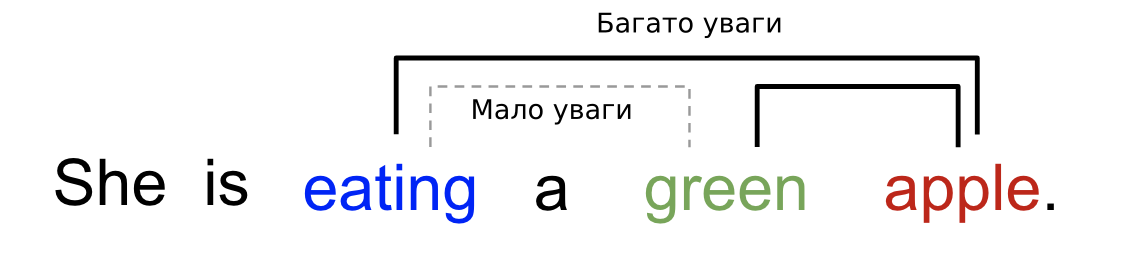
\includegraphics[width=0.75\textwidth]{sentence-example-attention.png}
    \caption{Одне слово ``поділяє увагу'' іншим словам по-різному}
    \label{fig:attend-example}
\end{figure}

Увагу при глибокому навчанні можна широко трактувати як вектор вагових
коефіцієнтів: для того, щоб передбачити або зробити висновок про один елемент,
наприклад, піксель на зображенні або слово в реченні, ми оцінюємо,
використовуючи вектор уваги, наскільки сильно він співвідноситься з іншими
елементами,
і приймає суму їх значень, зважену вектором уваги, як наближення
цілі \cite{attention}.

Механізм уваги народився, щоб допомогти запам’ятати довгі початкові
речення в машинному нейронному перекладі (МНП). Замість того,
щоб будувати єдиний вектор контексту із останнього прихованого стану
енкодера, підхід, винайдений увагою, полягає у створенні
скорочених шляхів між контекстним вектором та
всією вихідною послідовністю. Ваги цих з'єднань скорочення
можна підправити для кожного вихідного елемента.

Хоча вектор контексту має доступ до всієї початкової послідовності,
нам не потрібно турбуватися про забування.
Відповідність між джерелом та ціллю вивчається та контролюється
за допомогою контекстного вектора. По суті, вектор контексту
споживає три частини інформації:

\begin{enumerate}[label=--]
    \item прихований стан енкодеру;
    \item прихований стан декодеру;
    \item відповідність між входом та ціллю.
\end{enumerate}

\begin{figure}[H]
    \centering
    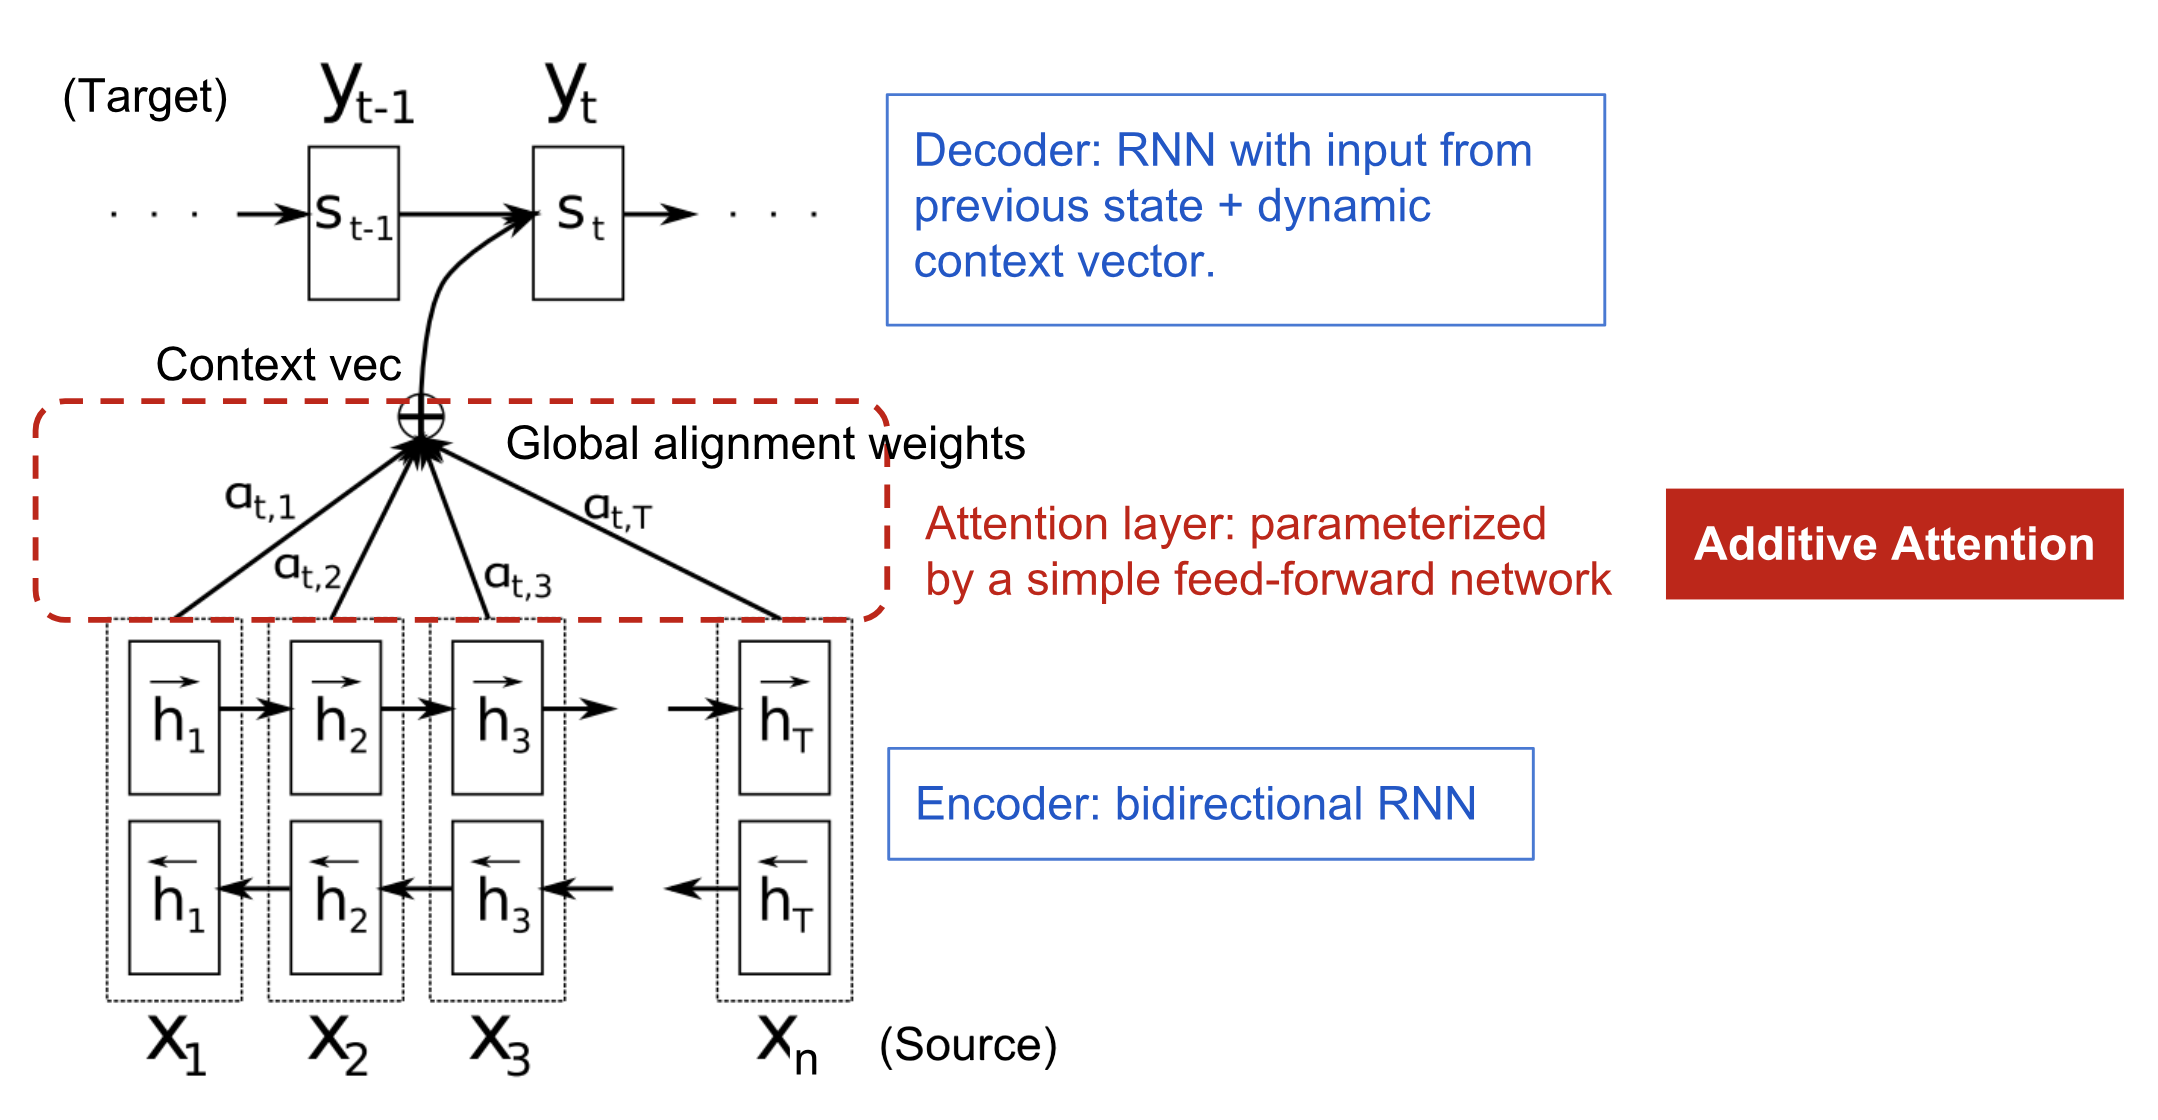
\includegraphics[width=1\textwidth]{encoder-decoder-attention.png}
    \caption{Архітектура рекурентної моделі з адитивною увагою}
    \label{fig:plot3}
\end{figure}

Механізм можна формально визначити так. Нехай є початкова послідовність
$x$ довжини $n$, і треба вивести цільову послідовність $y$
довжини $m$:

\begin{gather}
\begin{aligned}
    x &= [x_1,x_2, ..., x_n] \\
    y &= [y_1,y_2, ..., y_n]
\end{aligned}
\end{gather}

Тут енкодер -- це двонаправлена РНМ (або будь-яка інша РНМ) із прямим
прихованим станом $\overrightarrow{h_i}$ та зворотнім
$\overleftarrow{h_i}$. Звичайна конкатенація двох представляє стан
енкодера. Мотивація цієї операції
полягає в тому, щоб включити як попередні, так і наступні
слова до анотації одного слова.

\begin{equation}
    h_i = [\overrightarrow{h_i}^T;\overleftarrow{h_i}^T], i=1, ..., n
\end{equation}

Мережа декодера має прихований стан $s_t = f(s_{t-1},t_{t-1},c_t)$
для слова, що виводиться, на позиції $t$, $t = 1, ..., m$,
де контекстний вектор $c_t$ є сумою зважених прихованих станів
вхідної послідовності:

\begin{gather}
\begin{aligned}
    c_t          &= \sum^n_{i=1}\alpha_{t,i} h_i \\
    \alpha_{t,i} &= align(y_t,x_t) \\
    &= \frac{\exp(score(s_{t-1}, h_i))}{\sum^n_{i'=1}\exp(score(s_{t-1},h_{i'}))}
\end{aligned}
\end{gather}

Модель відповідності призначає оцінку $\alpha_{t,i}$
парі вхідних даних у позиції $i$ та виході у позиції $t$, ($y_t$, $x_i$),
залежно від того, наскільки вони співвідносяться. Множина
${α_{t,i}}$ -- це ваги, що визначають, наскільки кожен прихований стан
входу слід враховувати для кожного виводу.
У статті Багданау \cite{nn:attention} оцінка відповідності
$α$ параметризується мережею прямого пересилання
з єдиним прихованим шаром, і ця мережа навчається спільно з
іншими частинами моделі. Таким чином, функція оцінки
має такий вигляд, враховуючи, що $\tanh$ використовується як
нелінійна функція активації:

\begin{equation}
    score(s_t, h_i) = v^T_a \tanh(W_a [s_t;h_i])
\end{equation}
Де обидва $v_a$ та $W_a$ є матрицями вагів, які вивчаються
моделлю відповідності.

Існує декілька варіацій механізму
уваги \cite{attention:1} \cite{attention:2}, які змінюють
функцію вираховування відповідності. Вище
була використана аддитивна \cite{nn:attention} увага.

Архітектури, засновані на трансформерах, які в основному
використовуються для моделювання завдань на розуміння мови,
уникають використання рекурентності у нейронних мережах і замість
цього цілком довіряють механізмам самоуваги для побудови
глобальних залежностей між входами та виходами.

\section{Теоретичні дослідження}
\subsection{Модель}
% In order to perform classification, we use the standard approach of adding an extra learnable “classification token” to the sequence.
% https://stackoverflow.com/questions/58123393/how-to-use-transformers-for-text-classification

% Також у попередніх роботах були запропоновані методи, які об'єднують
% рекурентні і згорткові шари в одній моделі, для виконання задач
% багатоміткової класифікації \cite{nn:cnn-rnn}, опису зображень.

\section{Експериментальні дослідження}


\newpage
\renewcommand\bibname{ПЕРЕЛІК ДЖЕРЕЛ ПОСИЛАННЯ}
\begin{thebibliography}{9}
    \bibitem{latex:friends}
    What are TeX and its friends? [Електронний ресурс] – Режим доступу до ресурсу: https://www.ctan.org/tex.

    \bibitem{latex:oss-devs-latex}
    Gaudeul A. Do Open Source Developers Respond to Competition? The LATEX Case Study / Alex Gaudeul. // Review of Network Economics. – 2007.

    \bibitem{webhooks:define}
    Webhooks [Електронний ресурс]. – 2019. – Режим доступу до ресурсу: https://developer.atlassian.com/server/jira/platform/webhooks/.

    \bibitem{webhooks:good}
    Lindsay J. Web hooks to revolutionize the web [Електронний ресурс] / Jeff Lindsay. – 2007. – Режим доступу до ресурсу: https://web.archive.org/web/20180630220036/http://progrium.com/blog/2007/05/03/web-hooks-to-revolutionize-the-web/.
    
    \bibitem{transformers:repo}
    State-of-the-art Natural Language Processing for Jax, PyTorch and TensorFlow [Електронний ресурс] – Режим доступу до ресурсу: https://github.com/huggingface/transformers.

    \bibitem{flashtext:arxiv}
    Replace or Retrieve Keywords In Documents at Scale [Електронний ресурс]. – 2017. – Режим доступу до ресурсу: https://arxiv.org/abs/1711.00046.

    \bibitem{flashtext:repo}
    FlashText module [Електронний ресурс] – Режим доступу до ресурсу: https://github.com/vi3k6i5/flashtext.

    \bibitem{ahocorasik:wiki}
    Aho–Corasick algorithm [Електронний ресурс] – Режим доступу до ресурсу: https://en.wikipedia.org/wiki/Aho%E2%80%93Corasick_algorithm.

    \bibitem{attention}
    Weng L. Attention? Attention! [Електронний ресурс] / Lilian Weng // lilianweng.github.io/lil-log. – 2018. – Режим доступу до ресурсу: http://lilianweng.github.io/lil-log/2018/06/24/attention-attention.html.

    \bibitem{cortex-stuff}
    Hubel D. Receptive fields, binocular interaction and functional architecture in the cat’s visual cortex / D. Hubel, T. Wiesel. // The Journal of physiology. – 1962. – С. 106–154.

    \bibitem{cortex-equations}
    Hodgkin A. quantitative description of membrane current and its application to conduction and excitation in nerve / A. Hodgkin, A. Huxley. // The Journal of physiology. – 1952. – С. 500–544.

    \bibitem{rozenblatt}
    Rosenblatt F. The perceptron, a perceiving and recognizing automaton Project Para / Frank Rosenblatt. // Cornell Aeronautical Laboratory. – 1957.

    \bibitem{nn:peyre}
    Peyré G. Mathematics of Neural Networks [Електронний ресурс] / Gabriel Peyré – Режим доступу до ресурсу: https://mathematical-tours.github.io/book-basics-sources/neural-networks-en/NeuralNetworksEN.pdf.

    \bibitem{nn:backpropagation}
    Rumelhart D. Learning representations by back-propagating errors / D. Rumelhart, G. Hinton, R. Williams. // nature. – 1986. – С. 533–536.

    \bibitem{gradient-descend}
    Ruder S. An overview of gradient descent optimization algorithms / Sebastian Ruder. // arXiv preprint arXiv:1609.04747. – 2016.

    \bibitem{nn:multilayer-perceptrons}
    Grosse R. Lecture 5: Multilayer Perceptrons [Електронний ресурс] / Roger Grosse – Режим доступу до ресурсу: https://www.cs.toronto.edu/~mren/teach/csc411\_19s/lec/lec10\_notes1.pdf.
\end{thebibliography}

\newpage
\chap{Додаток 1}
% \centerline{\uppercase{\bf{Програмна реалізація}}}
%     \inputminted[breaklines,linenos=true]{python}{../../src/app.py}

% \chap{Додаток 2}
% \centerline{\uppercase{\bf{Результати роботи}}}
%     \begin{figure}[H]
%         \centering
%         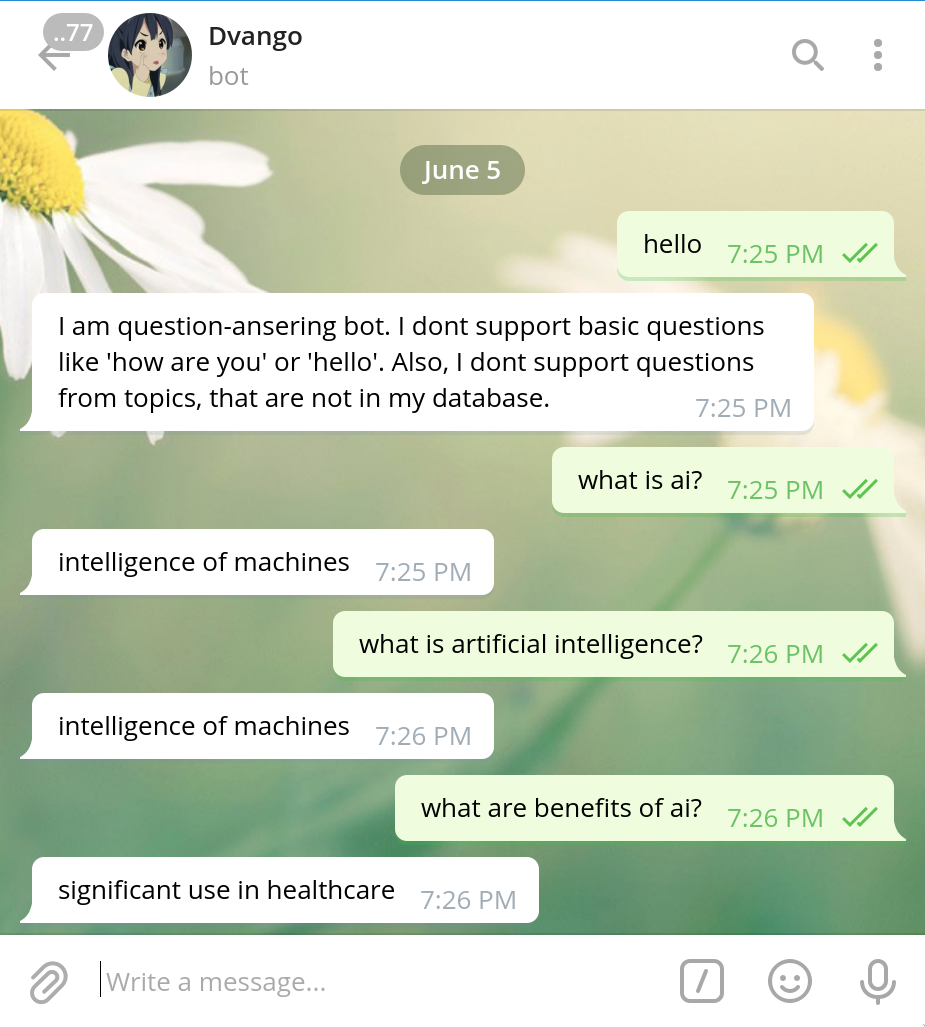
\includegraphics[width=0.75\textwidth]{f1.png}
%     \end{figure}
    
%     \begin{figure}[H]
%         \centering
%         
\includegraphics[width=0.75\textwidth]{f2.png}
%     \end{figure}

%     \begin{figure}[H]
%         \centering
%         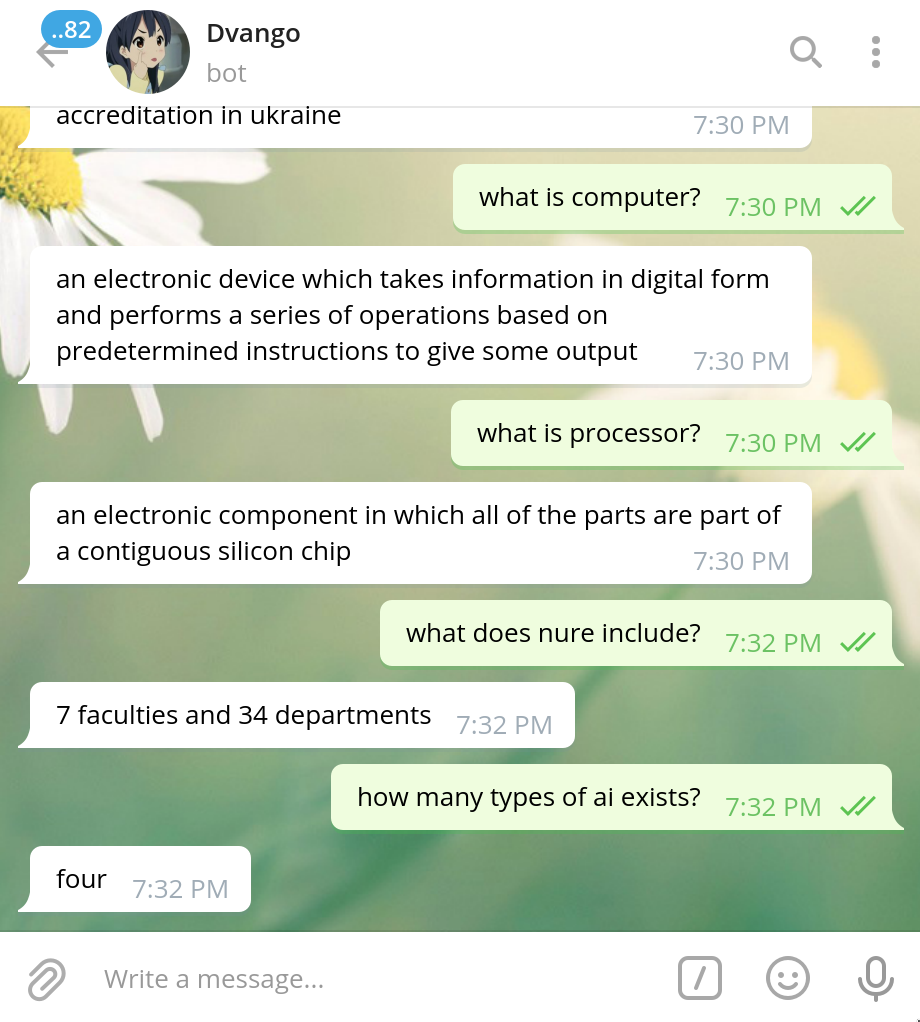
\includegraphics[width=0.75\textwidth]{f3.png}
%     \end{figure}
\end{document}


% \begin{figure}[H]
%     \centering
%     \includegraphics[width=0.75\textwidth]{rplot_iris.png}
%     \caption{Графік дерева вибірки Iris з дискретизацією через IG}
%     \label{fig:plot3}
% \end{figure}

% \begin{table}[H]
%     \centering
%     \begin{tabular}{ |c|c|c|c| } 
%      \hline
%      Мова   & \multicolumn{3}{c|}{Метод та датасет} \\ \hline
%             & Iris Thr. & Iris IG & SUSY \\ \hline
%      Python & 0.9333    & 0.9333  & 0.6799 \\ \hline
%      R      & 0.9333    & 0.9777  & 0.6594 \\ 
%      \hline
%     \end{tabular}
%     \caption{Порівняння точності класифікації}
%     \label{tab:t1}
% \end{table}
% \inputminted[breaklines,linenos=true]{scilab}{repl235.txt}
